\documentclass{beamer}
\usepackage{ctex, hyperref}
\usepackage[T1]{fontenc}
\usepackage{bookmark}
\usepackage{amsmath}
\usepackage{latexsym,amsmath,xcolor,multicol,booktabs,calligra}
\usepackage{graphicx,pstricks,listings,stackengine,subfigure,extpfeil}
\usepackage{wrapfig}
\author{Wangxianyi}
\usepackage{graphicx}
\usepackage{algorithm}
\usepackage{algpseudocode}
\usepackage{multirow}
\title{MAPDP: \newline Cooperative Multi-Agent Reinforcement Learning to Solve Pickup and
Delivery Problems}
\institute{LZU}
\date{\today}

\usepackage{NJUPT}

\def\cmd#1{\texttt{\color{red}\footnotesize $\backslash$#1}}
\def\env#1{\texttt{\color{blue}\footnotesize #1}}
\definecolor{deepblue}{rgb}{0,0,0.5}
\definecolor{deepred}{rgb}{0.6,0,0}
\definecolor{deepgreen}{rgb}{0,0.5,0}
\definecolor{halfgray}{gray}{0.55}

\lstset{
    basicstyle=\ttfamily\small,                                                                                                                                                                                                                                           
    keywordstyle=\bfseries\color{deepblue},
    emphstyle=\ttfamily\color{deepred},    % Custom highlighting style
    stringstyle=\color{deepgreen},
    numbers=left,
    numberstyle=\small\color{halfgray},
    rulesepcolor=\color{red!20!green!20!blue!20},
    frame=shadowbox,
}

\begin{document}

\kaishu
\begin{frame}
	\titlepage
\end{frame}

\begin{frame}
	\tableofcontents[sectionstyle=show,subsectionstyle=show/shaded/hide,subsubsectionstyle=show/shaded/hide]
\end{frame}


\section{Introduction}

\begin{frame}{Background Introduction}
	\begin{itemize}
		\item Vehicle Routing Problem (VRP) is crucial in various real-world applications such as express systems, industrial warehousing, and on-demand delivery.
		\item Cooperative Pickup and Delivery Problem (PDP) is a variant of VRP that plays a significant role in applications like on-demand delivery and industrial logistics.
		\item Challenges in solving cooperative PDP include structural dependency between pickup and delivery pairs and the need for effective cooperation among different vehicles.
		\item Existing solutions face difficulties in explicit modeling of dependencies and cooperation, leading to suboptimal performance.
	\end{itemize}
\end{frame}

\begin{frame}{Research Objectives}
	\begin{itemize}
		\item Explore the cooperative Pickup and Delivery Problem (PDP) with multiple vehicle agents using Multi-Agent Reinforcement Learning (MARL).
		\item Design a centralized MARL framework to generate cooperative decisions by capturing the inter-dependency of heterogeneous nodes.
		\item Train different agents based on communication embedding using a specially designed cooperative Advantage Actor-Critic (A2C) algorithm.
		\item Evaluate the effectiveness of the MAPDP framework on different datasets and compare its performance with existing baselines.
	\end{itemize}
\end{frame}

\begin{frame}{Overview of MAPDP Framework}
	\begin{itemize}
		\item MAPDP is a novel cooperative Multi-Agent Reinforcement Learning (MARL) framework designed to solve the Cooperative Pickup and Delivery Problem (PDP).
		\item The framework utilizes multi-agent cooperation to generate high-quality solutions by sharing a common context encoder and individual decoders for each vehicle agent.
		\item MAPDP learns to generate the next node to visit for each vehicle agent step by step and outputs a complete routing plan.
		\item Key components of MAPDP include paired context embedding to represent node dependencies, cooperative decoders for decision dependence, and a cooperative A2C algorithm for model training.
	\end{itemize}
\end{frame}

\section{Problem Formulation}

\begin{frame}{Introduction to Cooperative Pickup and Delivery Problem (PDP)}
	% \resizebox{\linewidth}{0.45\textheight}{ % 缩放以适应幻灯片宽度
	% 	\begin{minipage}{\textwidth} % 确保不超出幻灯片的宽度
	% 		\begin{align*}
	% 			 & \mathrm{min}&& \sum_{k=1}^{K}\sum_{i=0}^{2N}\sum_{j=1}^{2N+1}e_{ij}x_{ijk},                           && \text{(1)} \\
	% 			 & s.t.        && \sum_{k=1}^{K}\sum_{j=1}^{2N+1}x_{ijk}=1,\forall i\in[0,2N],                           && \text{(1)} \\
	% 			               && \sum_{k=1}^{K}\sum_{i=0}^{2N}x_{ijk}=1,\forall j\in[1,2N+1],                           && \text{(1)} \\
	% 			               && \sum_{i\in S^{\prime}}d_{i}\leq C_{k},\forall S^{\prime}\subseteq S,\forall k\in[1,K], && \text{(1)} \\
	% 			               && \sum_{j=1}^{2N+1}x_{i,jk}=\sum_{j=0}^{2N+1}x_{i+N,jk},\forall k\in[1,K],i\in[1,N],     && \text{(1)} \\                                                                                                                                                               \\
	% 			               && T_{i}\leq T_{i+N},\forall i\in[1,N].                                                   && \text{(1)} \\
	% 		\end{align*}
	% 	\end{minipage}
	% }
	\begin{itemize}
		\item Node Representation
		\item Node Pairing
		\item Spatial Distances
		\item Demand Volume
		\item Assignment to Vehicles
		\item Routing Decision
		\item Arrival Time
		\item Routing Sequence
	\end{itemize}
\end{frame}

\begin{frame}{Mathematical Modeling of Cooperative PDP}
	\centering
	\begin{align}
		\mathrm{min} \sum_{k=1}^{K}\sum_{i=0}^{2N}\sum_{j=1}^{2N+1}e_{ij}x_{ijk}
	\end{align}

	\begin{align}
		\sum_{k=1}^{K}\sum_{j=1}^{2N+1}x_{ijk}=1,\forall i\in[0,2N]
	\end{align}

	\begin{align}
		\sum_{k=1}^{K}\sum_{i=0}^{2N}x_{ijk}=1,\forall j\in[1,2N+1]
	\end{align}
	% \begin{figure}
	% 	\centering
	% 	\subfigure[]{
	% 		\begin{minipage}[b]{0.3\textwidth}
	% 			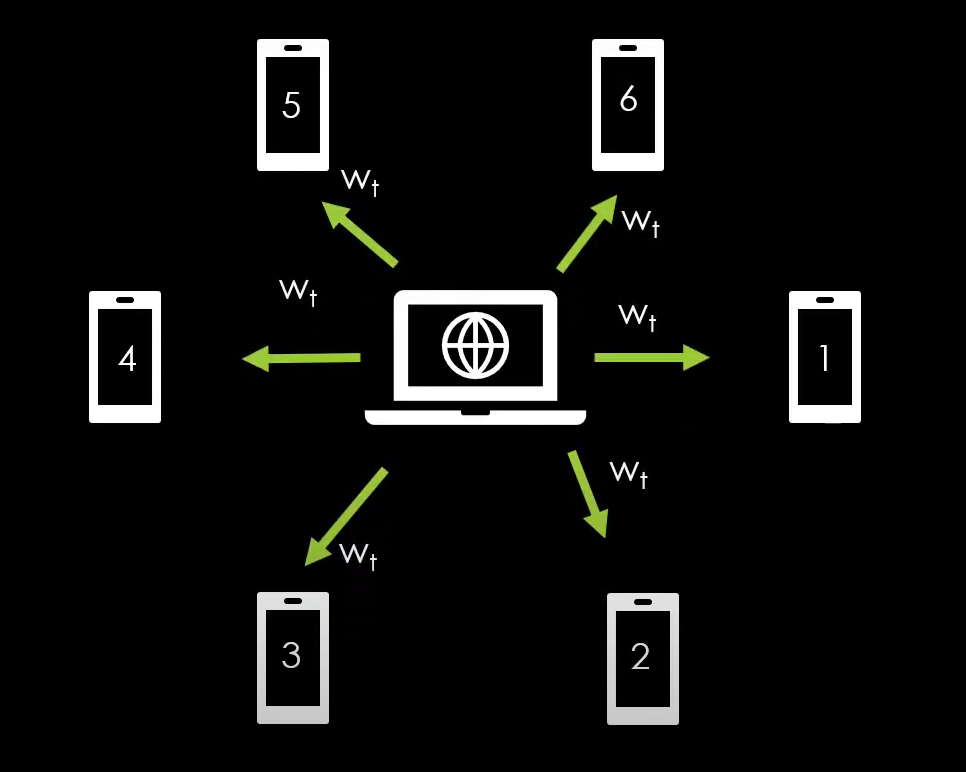
\includegraphics[width=1\textwidth]{fedavg_pic1.png}
	% 		\end{minipage}
	% 		\label{fig:grid_4figs_1cap_4subcap_1}
	% 	}
	% 	\subfigure[]{
	% 		\begin{minipage}[b]{0.3\textwidth}
	% 			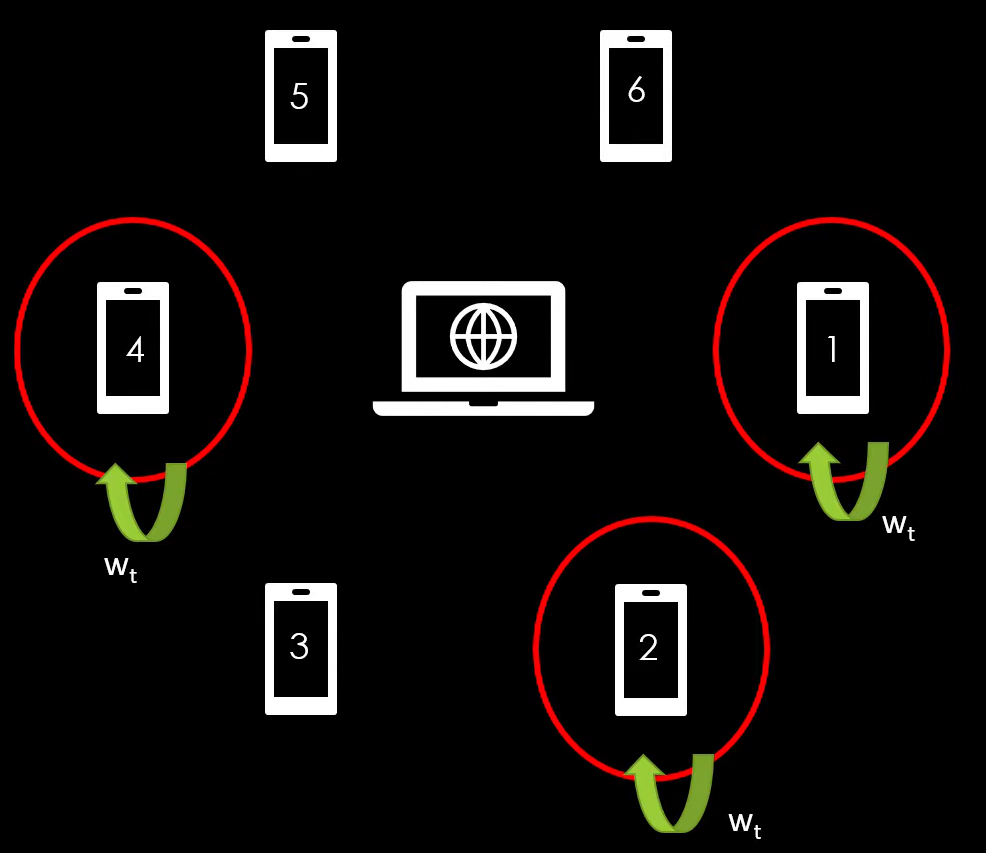
\includegraphics[width=1\textwidth]{fedavg_pic2.png}
	% 		\end{minipage}
	% 		\label{fig:grid_4figs_1cap_4subcap_2}
	% 	}
	% 	\\
	% 	\subfigure[]{
	% 		\begin{minipage}[b]{0.3\textwidth}
	% 			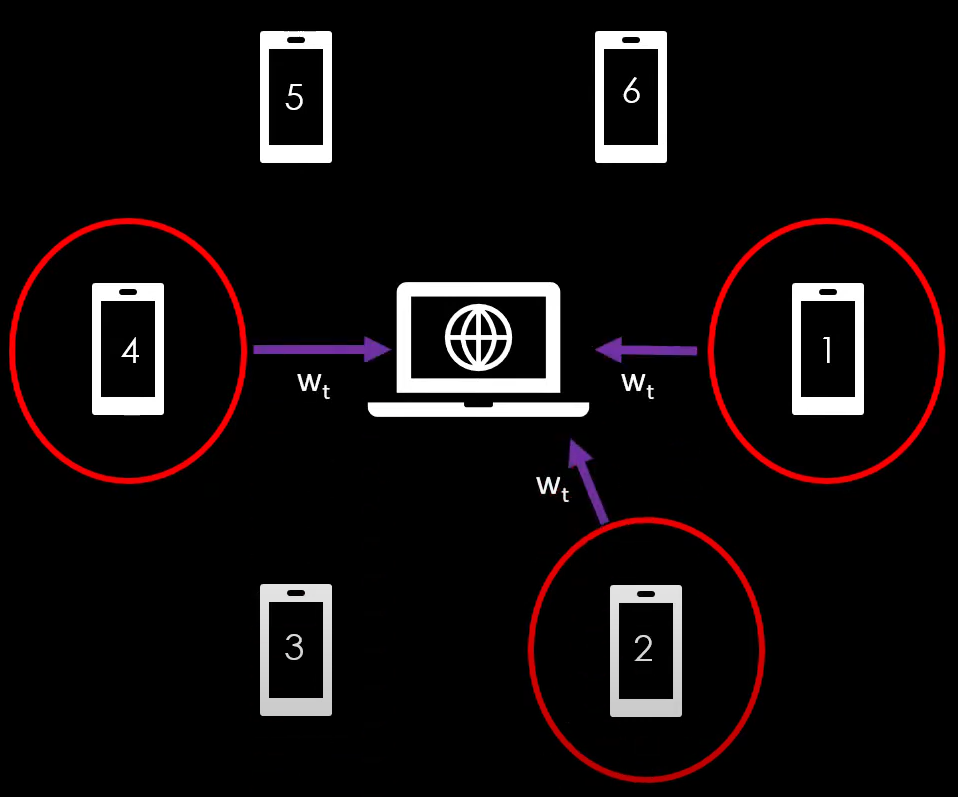
\includegraphics[width=1\textwidth]{fedavg_pic3.png}
	% 		\end{minipage}
	% 		\label{fig:grid_4figs_1cap_4subcap_3}
	% 	}
	% 	\subfigure[]{
	% 		\begin{minipage}[b]{0.3\textwidth}
	% 			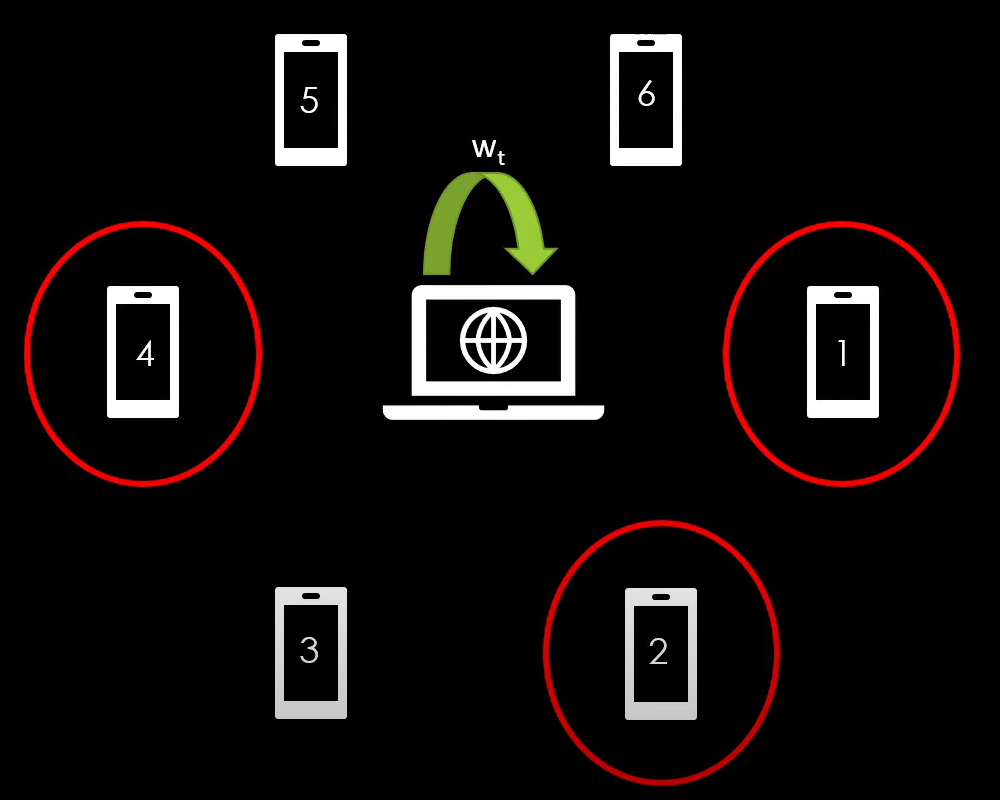
\includegraphics[width=1\textwidth]{fedavg_pic4.png}
	% 		\end{minipage}
	% 		\label{fig:grid_4figs_1cap_4subcap_4}
	% 	}
	% 	\caption{}
	% 	\label{fig:grid_4figs_1cap_4subcap}
	% \end{figure}
\end{frame}

\begin{frame}{Mathematical Modeling of Cooperative PDP}
	\begin{align}
		\sum_{i\in S^{\prime}}d_{i}\leq C_{k},\forall S^{\prime}\subseteq S,\forall k\in[1,K]
	\end{align}
	\begin{align}
		\sum_{j=1}^{2N+1}x_{i,jk}=\sum_{j=0}^{2N+1}x_{i+N,jk},\forall k\in[1,K],i\in[1,N]
	\end{align}
	\begin{align}
		T_{i}\leq T_{i+N},\forall i\in[1,N]
	\end{align}

\end{frame}
% \begin{frame}{Problem}
% 	There are two primary aspects of the algorithm;
% 	\begin{itemize}
% 		\item How to compute global/local loss function?
% 		\item How to compute global/local gradient calculation and update state
% 	\end{itemize}
% \end{frame}

% \begin{frame}{Objective Function}
% 	The objective function:
% 	\begin{align}
% 		\mathop{min}\limits_{\omega \in R^d}f(\omega)
% 	\end{align}
% 	\begin{align}
% 		f(\omega)=\frac{1}{n}\sum_{i=1}^{n}f_i(\omega)
% 	\end{align}
% 	Every client computes the loss function above with its local dataset
% 	Then these local loss scores are weighted-averaged
% 	\begin{align}
% 		f(\omega)=\sum_{k=1}^K\frac{n_k}{n}F_k(\omega)
% 	\end{align}

% 	\begin{align}
% 		F_k(\omega)=\frac{1}{n_k}\sum_{i \in P_k}^{n}f_i(\omega)
% 	\end{align}
% \end{frame}

% \begin{frame}{Optimize}
% 	\textbf{FederatedAveraging(or FedAvg)}\\
% 	Each client k locally takes one step of gradient descent on the global model with its local dataset.
% 	\begin{align}
% 		\forall k, \quad \omega_{t+1}\gets \omega_t-\eta g_k
% 	\end{align}
% 	Then the server takes a weighted average of the resulting models.
% 	\begin{align}
% 		\omega_{t+1}\gets \sum_{k=1}^{K} \frac{n_k}{n}\omega_{t+1}^k
% 	\end{align}
% \end{frame}

% \begin{frame}{Computation}
% 	(FedAvg) fits real world problems more.
% 	\begin{align}
% 		\omega^k \gets \omega^k-\eta \nabla F_k(\omega^k)
% 	\end{align}

% 	Computation is controlled by three key parameters for this approach
% 	\begin{itemize}
% 		\item C:The fraction of clients that perform computation  on each round.
% 		\item E:Number of training passes each client makes over its local dataset on each round.
% 		\item B:Local minibatch size used for the client updates.
% 	\end{itemize}
% \end{frame}

% \begin{frame}{Algorithm}

% 	\begin{figure}[htbp]
% 		\centering
% 		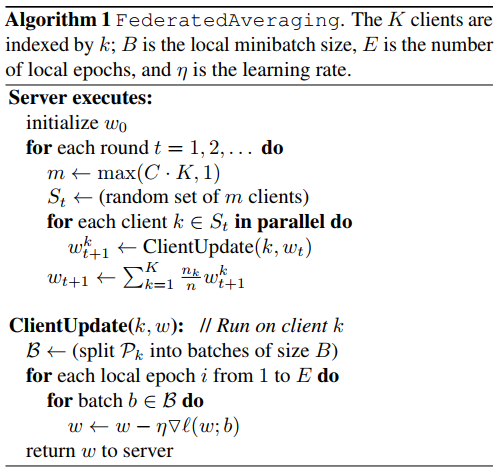
\includegraphics[scale=0.6]{alg.png}
% 		\caption{FederatedAveraging}
% 	\end{figure}
% \end{frame}

\section{Methodology}

\begin{frame}{Explanation of State, Action}
	\begin{itemize}
		\item State: The state of agent $k$ at step $t$ includes the remaining available capacity $C_k^t$ the current traveling trajectory $S_{k}^{t}.$ Specifically, the current location, i. e, the last node visited by agent $k$ is represented as $v_{I_{k}^{t}, \text{where }I_{k}^{t}\mathrm{~is~the}}$ node index. Note that $v_{I_{k}^{0}= v_{0} \mathrm{and~}C_{k}^{0}= C_{k}. \mathrm{In~the}}$ cooperative PDP setting, we assume that all vehicles can communicate via a centralized control so that all states are fully observable.
		\item Action: The action at step $t$ for vehicle agent $k$ is to determine a node as its next target, represented as $v(k,t).$
	\end{itemize}
\end{frame}

\begin{frame}{Explanation of Transition, Reward}
	\begin{itemize}
		\item Transition: The transition between adjacent states is to replace every agent to its target no0de as its current action. Then we update both the trajectory and the remaining capacity of each agent: $S_k^{t+1}=(S_k^t;\{v_{I_k^t}\}), C_k^{t+1}=C_k^t-d_{I_k^t}$,where ; means concatenating the partial solution with the new selected node.
		\item Reward: To optimize the overall routing solution quality, all agents share a common objective, which is to minimize the accumulated traveling distance of all agents in the entire episode. In each decision step, the one-step reward $r_k^t=-e_{I_k^t,I_k^{t+1}}$ is the negative of the length of the newly established arc. The final episode reward $R$ can be computed as $R=\sum_{k=1}^{k=K}\sum_{t=0}^{T-1}r_k^t$ where T is the decision step amount in a complete episode and $I_k^0=0$ means that all vehicles start from the depot $v_0$.
	\end{itemize}
\end{frame}
\begin{frame}{How Agents Learn to Collaborate in Solving PDP Problems}
	Model
	\begin{itemize}
		\item LSTM\cite{kim2016character}
	\end{itemize}
	Data distribution
	\begin{itemize}
		\item Balanced and IID version
		\item Unbalanced and non-IID version
	\end{itemize}
\end{frame}

% \begin{frame}{Experiment Results}

% 	% \begin{table}[h!]
% 	% 	Increasing Computation per client
% 	% 	\begin{center}
% 	% 		\small
% 	% 		\caption{Your first table.}
% 	% 		\begin{tabular}{c|c|c|c|c|c} % <-- Alignments: 1st column left, 2nd middle and 3rd right, with vertical lines in between
% 	% 			\textbf{MINST 2NN} & \textbf{E} & \textbf{B} & \textbf{u} & \textbf{IID} & \textbf{Non-IID} \\
% 	% 			\hline
% 	% 			FEDSGD             & 1          & $\infty$   & 1          & 1468         & 1817             \\
% 	% 			FEDAVG             & 10         & $\infty$   & 10         & 156(9.4x)    & 1100(1.7x)       \\
% 	% 			FEDAVG             & 1          & 50         & 12         & 144(10.2x)   & 1183(1.5x)       \\
% 	% 			FEDAVG             & 20         & $\infty$   & 20         & 92(16.0x)    & 957(1.9x)        \\
% 	% 			FEDAVG             & 1          & 10         & 60         & 92(16.0x)    & 831(2.2x)        \\
% 	% 			FEDAVG             & 10         & 50         & 120        & 45(32.6x)    & 881(2.1x)        \\
% 	% 			FEDAVG             & 20         & 50         & 240        & 39(37.6x)    & 835(2.2x)        \\
% 	% 			FEDAVG             & 10         & 10         & 600        & 34(43.2x)    & 497(3.7x)        \\
% 	% 			FEDAVG             & 20         & 10         & 1200       & 32(45.9x)    & 738(2.5x)        \\
% 	% 		\end{tabular}
% 	% 	\end{center}
% 	% \end{table}
% 	\begin{figure}[htbp]
% 		\centering
% 		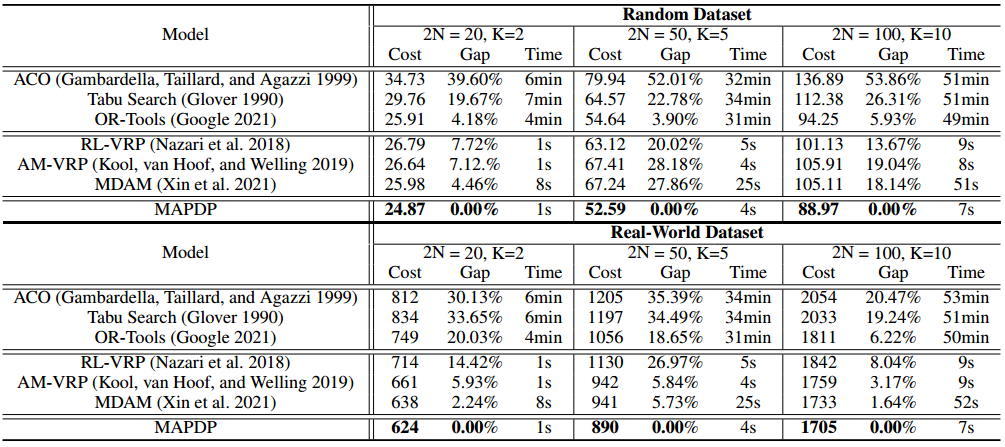
\includegraphics[scale=0.7]{table1.png}
% 		\caption{Effect of the client fraction C on the MNIST 2NN
% 			with E = 1 and CNN with E = 5.}
% 	\end{figure}
% 	C is set to 0.1 for all experiments. \\
% 	Computation increased by increasing E, decreasing B.
% \end{frame}

% \begin{frame}{Experiment Results}
% 	\begin{figure}[htbp]
% 		\centering
% 		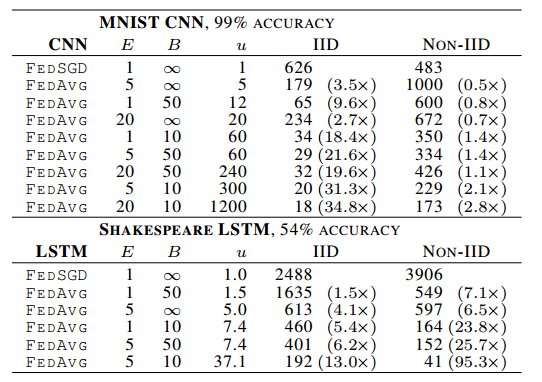
\includegraphics[scale=0.7]{table2.png}
% 		\caption{Effect of the client fraction C on the MNIST 2NN
% 			with E = 1 and CNN with E = 5.}
% 	\end{figure}
% \end{frame}

% \begin{frame}{Experiment Results}
% 	\begin{figure}[htbp]
% 		\begin{minipage}{0.6\textwidth}
% 			\centering
% 			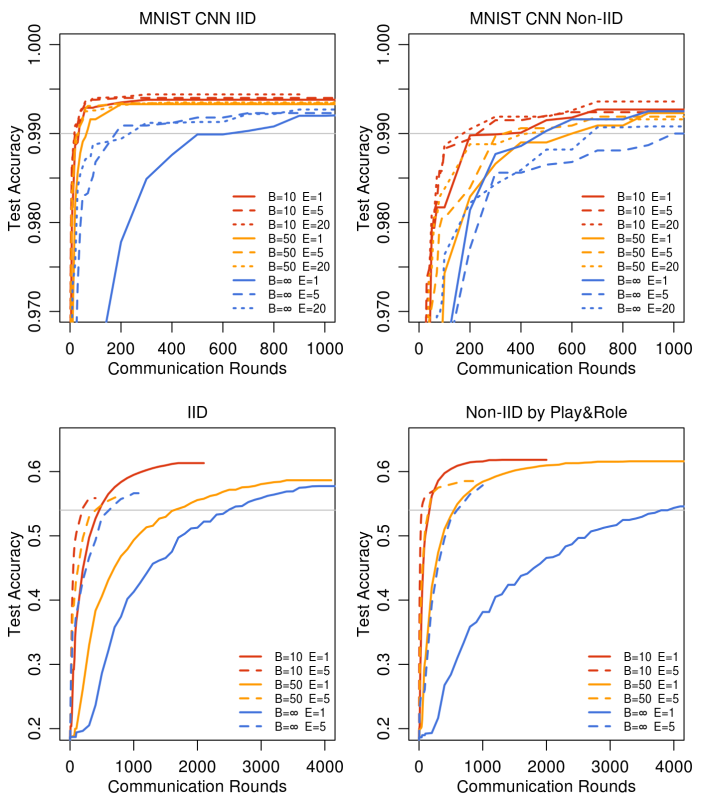
\includegraphics[scale=0.4]{line1.png}
% 		\end{minipage}%
% 		\hfill
% 		\begin{minipage}{0.4\textwidth}
% 			\caption{Test set accuracy vs. communication rounds
% 				for the MNIST CNN and Shakespeare LSTM  with
% 				C = 0.1 and optimized η. The gray lines show the target
% 				accuracies used in Table 4. }
% 		\end{minipage}
% 	\end{figure}
% \end{frame}
% \begin{frame}{Experiment Results}
% 	\begin{figure}[htbp]
% 		\centering
% 		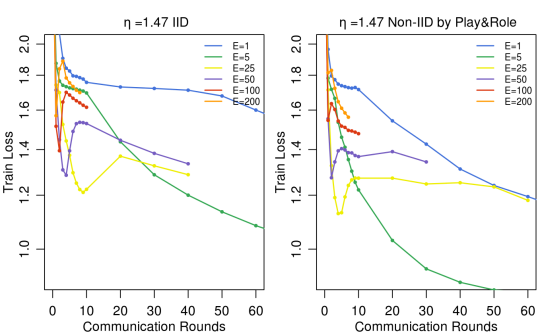
\includegraphics[scale=0.7]{table3.png}
% 		\caption{The effect of training for many local epochs between averaging steps, fixing B = 10 and C = 0.1 for
% 			the Shakespeare LSTM with a fixed learning rate η = 1.47.}
% 	\end{figure}
% \end{frame}

% \begin{frame}{Experiment Conclusion}
% 	\begin{itemize}
% 		\item Using extreme non IID data to train the model, FedAvg can also perform better than FedSGD, indicating that the FedAvg algorithm may have strong robustness.
% 		\item FedAvg has higher accuracy than FedSGD on the test set, and the author speculates that FedAvg produces a dropout like regularization effect.
% 		\item When larger, the accuracy of FedAvg algorithm convergence will decrease, or even not converge.
% 	\end{itemize}
% \end{frame}

\section{MAPDP}

\begin{frame}{Overview of MAPDP Framework}
	\begin{figure}
		\centering
		\hspace{-1.2cm} % Adjust the value to move the image to the left
		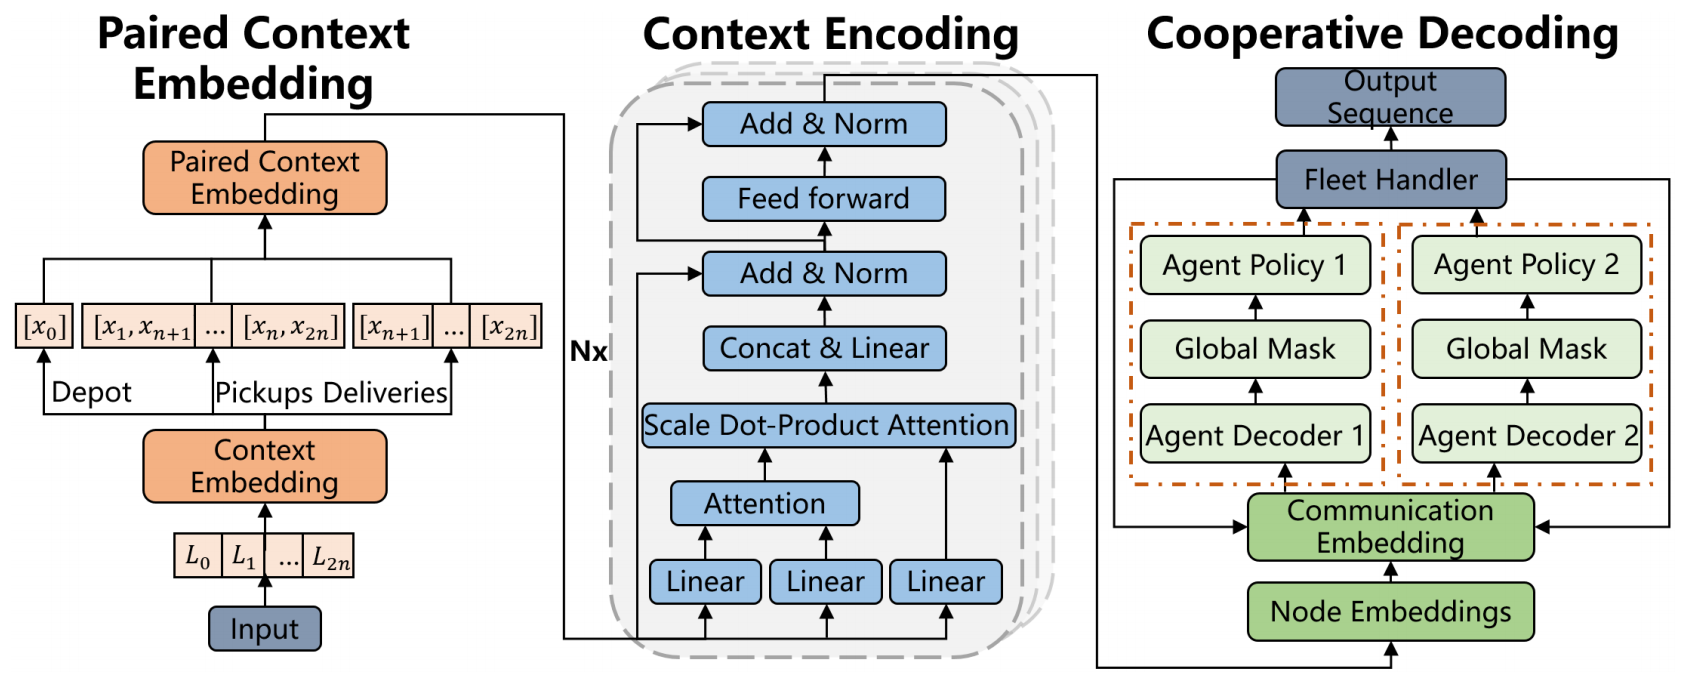
\includegraphics[scale=0.199]{model_structure.png}
		\caption{MAPDP Framework}
	\end{figure}
\end{frame}

\begin{frame}{Paired Context Embedding}
	\begin{align}
		h_i^0=\begin{cases}W_0^xx_i+b_0^x,&i=0,\\W_p^x[x_i;x_{i+N}]+b_p^x,&1\le i\le N,\\W_d^xx_i+b_d^x,&N+1\le i\le2N,\end{cases}
	\end{align}

	\begin{align}
		\hat{h_{i}}=BN^{\ell}(h_{i}^{\ell-1}+MHA_{i}^{\ell}(h_{1}^{\ell-1},h_{2}^{\ell-1},\cdots h_{2N}^{\ell-1})),
	\end{align}

	\begin{align}
		h_{i}^{\ell}=BN^{\ell}(\hat{h_{i}}+FF^{\ell}(\hat{h_{i}})).
	\end{align}
\end{frame}


\begin{frame}{Context Encoding}
	\begin{align}
		Q_i^h,K_i^h,V_i^h=W_Q^hh_i,W_K^hh_i,W_V^hh_i,
	\end{align}

	\begin{align}
		A_i^h=softmax(Q_i^h{K^h}^T/\sqrt{d_k})V_j^h,
	\end{align}

	\begin{align}
		MHA_i=Concat(A_i^1,A_i^2,...,A_i^H)W_O,
	\end{align}
\end{frame}

\begin{frame}{Cooperative Multi-Agent Decoders}
	\begin{align}
		Comm^t=[h_{I_1^t};C_1^t;h_{I_2^t};C_2^t;...;h_{I_K^t};C_K^t]
	\end{align}

	\begin{align}
		g_{k}^{t}=MHA_{k,(c)}(h_{1},h_{2},...,h_{2N}),
	\end{align}

	\begin{align}
		Q_{k}^{t},K_{k,i}^{t}=W_{Q,k}g_{k}^{t},W_{K,k}h_{i},
	\end{align}

	\begin{align}
		u_{k,i}^{t}=Dtanh(Q_{k}^{t}{}^{T}K_{k,i}^{t}/\sqrt{d_{k}}),
	\end{align}

	\begin{align}
		p_{\theta_{k},\phi}(v(k,t))=softmax(Mask^{t}(u_{k,i}^{t})),
	\end{align}

\end{frame}

\section{Experiments}

\begin{frame}{Evaluation Results on Different Datasets}
	\begin{figure}
		\centering
		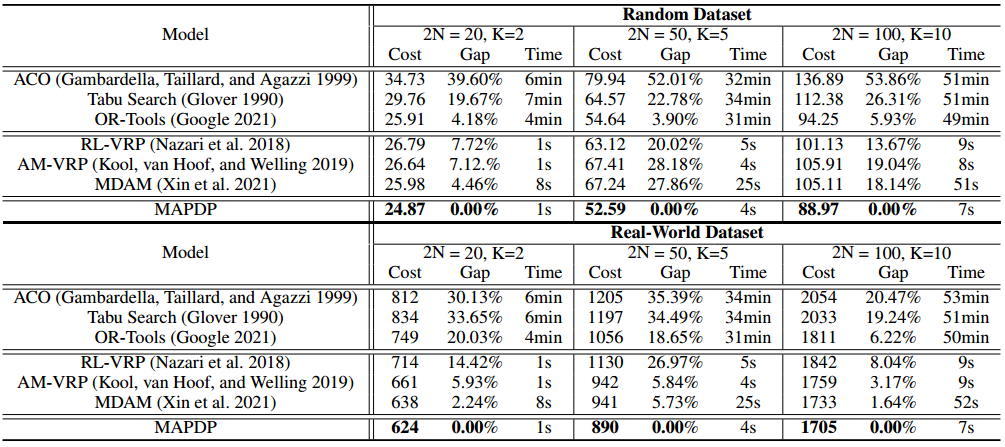
\includegraphics[scale=0.3]{table1.png}
		\caption{Comparison of Different Models on Random and Real-World Datasets}
	\end{figure}
\end{frame}

\begin{frame}{Performance Comparison with Other Methods}
	\begin{figure}
		\centering
		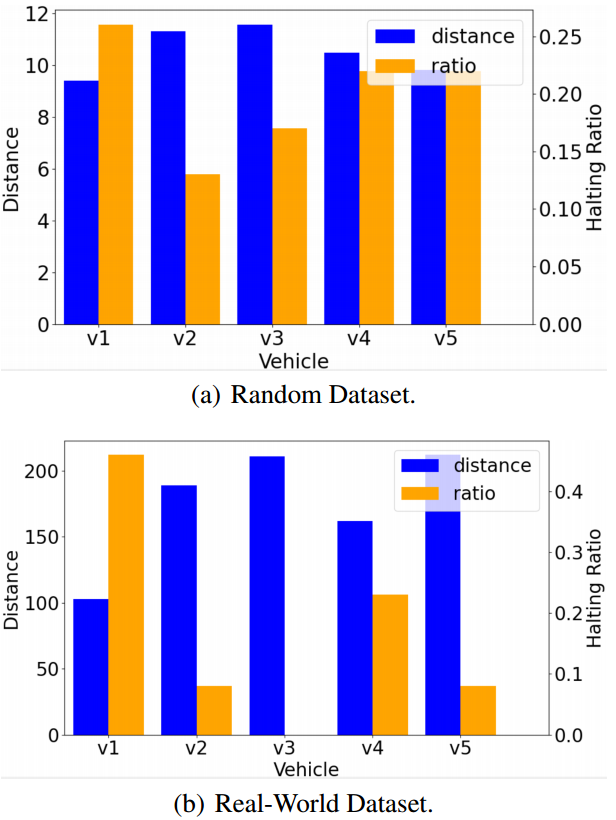
\includegraphics[scale=0.2]{graph.png}
		\caption{ Case studies on vehicle cooperation analysis from two datasets.}
	\end{figure}
\end{frame}

\section{Conclusion}

\begin{frame}{Conclusion}
	\begin{itemize}
		\item The proposed MAPDP framework leverages Multi-Agent Reinforcement Learning (MARL) to effectively solve the Cooperative Pickup and Delivery Problem (PDP) by capturing dependencies and promoting cooperation among multiple vehicles.
		\item MAPDP outperforms existing baselines by at least 1.64% in all experiment settings, demonstrating its superior performance in generating high-quality solutions for PDP.
		\item The centralized MARL framework, paired context embedding, cooperative decoders, and cooperative A2C algorithm collectively contribute to the success of MAPDP in addressing the challenges of PDP.
		\item Future research directions may include exploring scalability of MAPDP to larger problem instances, incorporating real-time constraints, and adapting the framework to dynamic environments.
	\end{itemize}
\end{frame}

\section{References}

\begin{frame}[allowframebreaks]
	\bibliography{ref}
	\bibliographystyle{njupt}
\end{frame}

\begin{frame}
	\begin{center}
		{\Huge \calligra Thanks!}
	\end{center}
\end{frame}

\end{document}